\chapter{疼痛的药物治疗}

\section{疼痛概述}

1979年世界卫生组织和1986年国际疼痛研究协会(International Association
for the Study
Pain,IASP)为疼痛所下的定义是“疼痛是组织损伤或潜在组织损伤所引起的不愉快感觉和情感体验”。

对患者而言,疼痛一方面是机体面临损害或疾病产生的信号,另一方面又是影响生活质量的重要因素之一。提醒患者应加以重视,及早就医,积极治疗以防机体遭受更大和更长久的损害。对医师而言,疼痛既是机体对创伤或疾病的反应,也是疾病的症状。急性疼痛起病急,常伴有心血管、呼吸、消化以及代谢、内分泌甚至免疫功能的改变。而慢性疼痛持续数月以上,常可降低食欲,影响睡眠,导致抑郁、焦虑等生理、心理和社会功能的改变。因此,疼痛需要及早治疗,必须合理应用镇痛药,缓解疼痛和减轻患者痛苦。

1995年美国疼痛学会主席JamesCampbell提出“将疼痛列为血压、脉搏、呼吸、体温之外的第五大生命体征”。在2000年欧洲疼痛大会和2001年亚太地区疼痛论坛上提出“消除疼痛是患者的基本权利”。在2002年第10届国际疼痛研究协会(IASP)大会上,与会专家达成基本共识,即慢性疼痛是一种疾病。2004年IASP确定10月11日是第一个“世界镇痛日”。

从医学伦理学和尊重人权的角度出发,每个医务工作者都应充分认识到患者有陈述疼痛、表达疼痛程度、得到完全镇痛、受到尊重并得到心理和精神上支持的权利和知情权。

\subsection{病因}

疼痛通常由导致组织损伤的各种伤害性刺激引起,包括物理性刺激(如刀割、棒击、电流和高温等)、化学性刺激(如强酸、强碱等)和生物性刺激(如蚊虫、蜂类叮蛰等)。此外,组织细胞炎症或损伤时释放入细胞外液中的钾离子、5-羟色胺、乙酰胆碱、缓激肽、前列腺素和组胺等生物活性物质亦可引起疼痛或痛觉过敏。

\subsection{发病机制}

关于疼痛的发生机制,早在1965年人们就提出了疼痛的闸门控制学说。该学说认为脊髓后角胶质中的某些神经细胞对疼痛信息的传递具有闸门作用,控制着疼痛信息向中枢传递,其本身也受周围神经粗、细传入纤维活动和高级中枢下行控制作用的影响。因而,任何使细纤维活动增强和(或)粗纤维活动减弱的因素均可导致疼痛。1970年,人们又进一步发现轻度电刺激中脑导水管周围灰质或向该处注射微量吗啡,可引起极明显的镇痛效果,并据此提出内源性疼痛抑制系统的概念。随后又发现导水管周围灰质中的神经细胞含有丰富的阿片肽受体,其周围存在大量的阿片肽(opioid
peptides)。现在认为,阿片受体和阿片肽共同组成了机体的抗痛系统。内源性阿片肽(如脑啡肽)可激动感觉神经突触前、后膜上的阿片受体,通过G-蛋白耦联机制,抑制腺苷酸环化酶,促进\ce{K^+}
外流、减少\ce{Ca^2+}
内流,使突触前膜递质释放减少、突触后膜超级化,最终减弱或阻滞痛觉信号的传递,产生镇痛作用。除内源性阿片肽及其受体外,5-羟色胺、前列腺素等递质及其相应的受体也参与下行控制或内源性疼痛控制系统。在成人,疼痛还可由心理原因引起,而无明显直接的物质基础。一般来说,疼痛易受注意、暗示和期待等心情的影响,一个人的既往经历和当时的情境均可给疼痛感受带来很大的影响。

\subsection{临床表现}

疼痛的表现复杂,这与疼痛的发生部位、影响因素和体位等均有关系。一般来说,疼痛部位多为病变或损伤所在部位,如胸痛、腹痛、腰背痛或关节痛等。疼痛性质有胀痛、闷痛、刺痛、切割痛、灼痛和绞痛等;疼痛程度有轻微疼痛至剧烈疼痛;持续时间有阵发性(1~5min)疼痛,也有持续性(数小时或更长)疼痛;某些体位可使疼痛加剧或减轻,有可能成为诊断的线索;疼痛的伴发症状可有发热、寒战、恶心、呕吐甚至休克等,伴随症状还可有焦虑、睡眠紊乱、食欲减退、便秘、个性改变等自主神经功能障碍,以及社会、家庭、心理多方面不适应的心理障碍,并可引发交感神经系统功能异常。

\subsection{分类}

\subsubsection{按起病缓急、病程长短分类}

(1)急性疼痛:有明确的开始时间,持续时间较短,常用的镇痛方法可控制疼痛,如软组织及关节急性损伤性疼痛、手术后疼痛、产科疼痛、痛风等。

(2)慢性疼痛:通常由慢性病理过程造成,逐渐发生,开始时间不很明确,并可能持续加重。如软组织及关节劳损性或退变性疼痛、椎间盘源性疼痛、神经源性疼痛等。

\subsubsection{按疼痛程度分类}

(1)微痛或似痛非痛:常与其他感觉复合出现,如痒、酸痛、沉重、不适感等。

(2)轻度疼痛的痛:反应较轻,常不影响正常的工作和生活。

(3)中度疼痛的痛:反应较强烈,能影响机体的正常活动和功能发挥。

(4)剧痛的痛:反应剧烈,难以忍受,可导致昏厥,应采取紧急救治措施。

\subsubsection{按疼痛性质分类}

可有钝痛、酸痛、胀痛、闷痛、锐痛、刺痛、切割痛、灼痛和绞痛等,也可有钻顶样痛、爆裂样痛、跳动样痛、撕裂样痛、牵拉样痛和压榨样痛等。

\subsubsection{按病理生理学角度分类}

(1)伤害性疼痛:是对组织损伤产生的一种病理生理过程,是机体对潜在组织损伤的一种保护性指示信号。

(2)神经病理性疼痛:通常定位较差,多较为稳定,也可表现为间断性针刺、撕裂感,或表现为感觉迟钝、麻木、感觉过敏或感觉异常。

(3)混合性疼痛:兼有上述两种性质的复杂疼痛,通常表现为慢性疼痛或者急性疼痛,治疗效果不理想。

\subsubsection{按疼痛来源分类}

(1)躯体疼痛:疼痛部位明确,如临床上手术后疼痛或躯体损伤后疼痛。

(2)内脏疼痛:定位常不明确,且经常扩散到相应的皮肤区域或形成皮肤痛觉过敏带,典型的内脏痛如胆绞痛、心绞痛。

(3)神经疼痛:癌肿浸润或治疗引起的神经末梢或中枢神经系统受损所致,表现为烧灼样、钳夹样的阵发性疼痛,往往伴有感觉或运动功能丧失。

\subsection{疼痛的诊断与评估}

诊断疼痛性疾病时,首先要明确疼痛诊断的内容和诊断的思路。疼痛诊断的程序和内容主要包括采集病史、临床检查、疼痛评估结果,最后做出疼痛的诊断和鉴别诊断。

\subsubsection{详细询问病史}

疼痛患者病史的采集:除采集一般病史外,重点询问疼痛的特征,疼痛首次出现的时间、环境、活动动态、疼痛部位、疼痛时间、疼痛程度、疼痛性质以及与体位的关系、影响因素、发作规律(持续时间、间隔时间,疼痛加重缓解原因)、治疗过程、治疗方法及效果等。系统且重点地采集病史,对疼痛的诊断很有价值,约半数以上的疼痛病例可根据病史做出诊断。

\subsubsection{体格检查、实验室检查和影像学检查}

疼痛的体格检查包括望诊、触诊、叩诊、听诊,在脊柱四肢还应该包括动量诊,必要时还需进行神经病学检查。

应酌情进行实验室检查,如血常规、尿常规及尿液检查、电解质、红细胞沉降率、血生化等,可提高诊断的准确性。

影像学检查,如X线、CT、MRI和超声检查等,也常具有重要诊断价值。

\subsubsection{疼痛强度评估}

疼痛是患者的一种主观感受,因此疼痛强度的评估并没有客观的医疗仪器可供选择,主要依靠患者的主观描述。目前常用的疼痛评估方法有以下几种。
\paragraph{视觉模拟评分法(Visual Analogue Scale,VAS)}

VAS基本的方法是使用一条游动标尺,正面是无刻度10cm长的滑道,“0”端和“10”端之间有一个可以滑动的标定物,“0”分表示无痛,“10”分表示难以忍受的最剧烈的疼痛,背面有“0~10”的刻度。使用时,将有刻度的一面背向患者,患者根据疼痛的强度滑动标定物至相应的位置,疼痛测量尺的背面有具体的刻度,根据标定物的位置可以直接读出疼痛程度指数。临床评定以0~2分为“优”,3~5分为“良”,6~8分为“可”,>8分为“差”。VAS简单易行、有效,相对比较客观且敏感。在表达疼痛强度时,是一种较少受到其他因素影响的测量方法。一般VAS方法用于8岁以上,能够正确表达自己感受和身体状况的患者。
\paragraph{疼痛强度简易描述量表(Verbal Rating Scale,VRS)}

本方法是将疼痛测量尺与口述描绘评分法相结合构成,特点是将描绘疼痛强度的词汇通过疼痛测量尺图形表达,使描绘疼痛强度的词汇梯度更容易使患者理解和使用。在使用该方法时,观察者应注意患者在表达疼痛强度时会受到情绪的影响,要正确对待患者的情绪化因素并进行评价。

0级:无疼痛。

I级(轻度):有疼痛但可忍受,生活正常,睡眠无干扰。

II级(中度):疼痛明显,不能忍受,要求服用镇痛药物,睡眠受干扰。

III级(重度):疼痛剧烈,不能忍受,需用镇痛药物,睡眠受严重干扰可伴自主神经紊乱或被动体位。
\paragraph{数字疼痛强度量表(Numerical Rating Scale,NRS)}

NRS是VAS方法的一种数字直观的表达方法,其优点是较VAS方法更为直观。患者被要求用数字(0~10)表达出感受疼痛的强度,由于患者易于理解和表达,明显减轻了医务人员的负担,是一种简单有效和最为常用的评价方法,通常可用疼痛与睡眠的关系提示疼痛的强度。若疼痛完全不影响睡眠,疼痛应评为<4分,为轻度痛;若疼痛影响睡眠但仍可自然入睡,疼痛应评为4~6分,为中度痛;若疼痛导致不能睡眠或睡眠中痛醒,需用镇痛药物或其他手段辅助帮助睡眠,疼痛应评为7~10分,为重度痛。此法的不足之处,是患者容易受到数字和描述字的干扰,降低了其灵敏性和准确性。NRS方法可以以口述或书面的形式使用,也可用于生活质量的评价。NRS方法可以教会患者及其家属使用,在评价疼痛治疗效果时,患者在家中能够详细记录每天的动态变化,利于对比治疗前后疼痛强度的变化,为治疗提供参考依据。
\paragraph{疼痛强度Wong-Baker脸谱量表(Face Rating Scale,FRS)}

FRS由6张从微笑直至流泪的不同表情的面部像形图组成,适用于交流困难,如儿童(3~6岁)、老年人、意识不清或不能用言语表达的患者,如图\ref{fig20-1}所示。

\begin{figure}[!htbp]
 \centering
 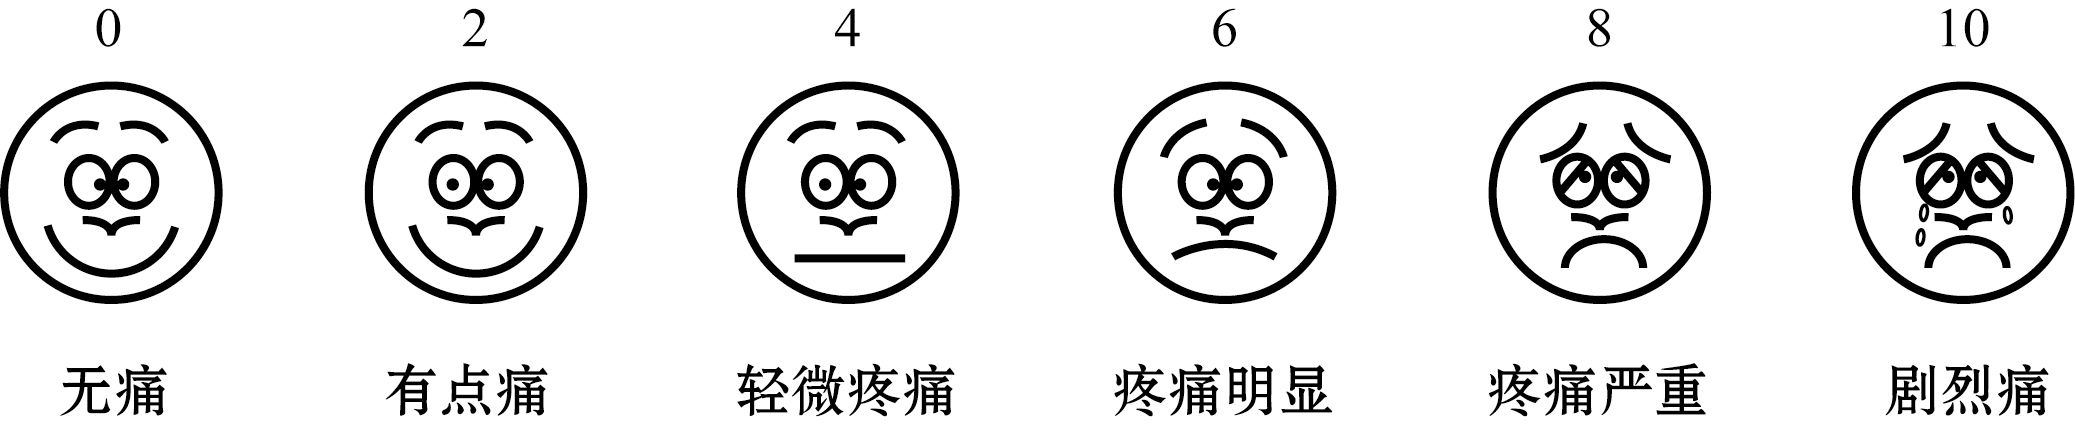
\includegraphics[width=.7\textwidth]{./images/Image00025.jpg}
 \captionsetup{justification=centering}
 \caption{疼痛强度脸谱}
 \label{fig20-1}
  \end{figure} 

\subsection{疼痛治疗原则}

\subsubsection{疼痛治疗的基本原则}

规范化疼痛处理(good pain
management,GPM)是近年来倡导的镇痛治疗新观念,唯有强调规范化才能有效提高疼痛的诊疗水平,减少疼痛治疗过程中可能出现的并发症。
\paragraph{明确治疗目的}

缓解疼痛,改善功能,提高生活质量。包括身体状态、精神状态、家庭、社会关系的维护和改善。
\paragraph{制定治疗计划}

治疗计划的制定要考虑疼痛强度、疼痛类型、基础健康状态、合并疾病以及患者对镇痛效果的期望和对生活质量的要求。规范化疼痛治疗原则为:有效消除疼痛,最大限度地减少不良反应,把疼痛治疗带来的心理负担降至最低,全面提高患者的生活质量。规范化治疗的关键是遵循用药和治疗原则。控制疼痛的标准是:数字评估法的疼痛强度小于3或达到0;24h内突发性疼痛次数小于3次。
\paragraph{处理不良反应}

对不良反应的处理,要采取预防为主,镇痛药与控制不良反应药应合理配伍,同等考虑。此外,要重视对心理、精神问题的识别和处理。
\paragraph{采取有效的综合治疗}

采用多种形式综合疗法治疗疼痛。一般以药物治疗为主,此外还有非药物治疗。主要镇痛药物为NSAIDs和阿片类镇痛药。对于轻度疼痛可应用非甾体抗炎止痛药;对中度疼痛主要应用弱阿片镇痛药及其复方制剂;对重度疼痛,弱阿片镇痛药无效时可采用吗啡等强效阿片类药。在治疗时可根据具体情况应用辅助药,如抗抑郁药、抗惊厥药等。对癌性疼痛患者,应遵循世界卫生组织提出的三阶梯镇痛原则。非药物疗法可在慢性疼痛治疗全过程中任何一时间点予以使用,可供选用的方法有外科疗法、神经阻滞疗法、神经毁损疗法和神经刺激疗法等。药物疗法与非药物疗法宜结合使用。

\subsubsection{药物治疗原则}

用药前应尽量明确病因,同时应积极对因治疗;原因不明者慎用镇痛药,以免掩盖症状、延误诊治。严禁滥用阿片类镇痛药。
\paragraph{选择适当的药物和剂量}

镇痛药物主要为NSAIDs和阿片类药物,应基于患者的疼痛类型和疼痛强度与当前治疗的相互作用而定。如癌痛属长期治疗计划,应按WHO的三阶梯治疗方案来指导用药。
\paragraph{选择给药途径}

应以无创给药或口服为首选途径。有吞咽困难和透皮贴剂禁忌证的,可选择经舌下含化或经直肠给药;仍无明显改善者可经肌内或静脉注射给药;产生难以控制的不良反应时可选用椎管内给药或复合局部阻滞疗法。
\paragraph{制定适当的给药时间}

依据药物不同的药动学特点来制定合适的给药间期。定时给药不仅可提高镇痛效果,还可减少不良反应。如各种盐酸盐或硫酸盐控释片的镇痛作用在用药后1h出现,2~3h达高峰,持续作用12h;而静脉给药可在5min内起效,持续1~2h。而定时给药是非常重要的,如芬太尼透皮贴剂的镇痛作用在6~12h起效,持续72h,每3d给药1次即可。
\paragraph{调整药物剂量}

在治疗之初要调整药物剂量。如患者突发性疼痛反复发作,需根据个体耐受情况不断调整追加药物剂量,增加幅度一般为原用剂量的25%~50%,最多不超过100%,以防各种不良反应造成危害。对于因其他辅助性治疗使疼痛已经减轻的患者,可逐渐下调药物剂量,一般每天减少25%~50%,但应在保证镇痛效果良好的基础上调整。当出现不良反应而需调整药物剂量时,应首先停药1或2次,再将剂量减少50%~70%,然后加用其他种类的镇痛药,逐渐停用有不良反应的药物。
\paragraph{处理不良反应}

应密切观察疼痛缓解程度和身体反应,采取必要措施减轻药物不良反应,避免药物依赖性。
\paragraph{善用辅助治疗}

辅助治疗的方法应依不同疾病、不同类型的疼痛而定。一般包括辅助药物和非药物疗法,如抗抑郁药、神经阻滞疗法等;通过联合治疗,可达到增强镇痛效果、减少镇痛药剂量、减轻镇痛药不良反应等目的。

总之,疼痛治疗时,选用多种药物联合应用、多种给药途径交替使用、按时用药、个体化用药,可提高镇痛效果。但在药物选择上应予以重视,避免盲目联合用药,力争用最少的药物、最小的剂量来达到满意的镇痛效果。

\section{慢性疼痛的治疗}

国际疼痛研究会(IASP)将慢性疼痛定义为“超过正常的组织愈合时间(一般为3个月)的疼痛”,但就实际而言,一般认为持续超过6个月的疼痛才算慢性疼痛。慢性疼痛的特点是病因复杂,常与其基础病变不相符或没有可解释的器质性病变,其发生、发展、持续加重与心理因素密切相关。根据病因可分为非癌性疼痛和癌性疼痛,有些还属于顽固性慢性疼痛,如三叉神经痛、带状疱疹后遗神经痛、幻肢痛、癌痛等。目前主要治疗方法有药物治疗、神经阻滞、外科手术治疗、心理治疗和其他治疗如针刺、物理疗法等。

\subsection{药物治疗原则}

慢性疼痛治疗应遵循WHO用于癌痛治疗的三阶梯镇痛原则。

\subsubsection{口服给药}

尽可能采用口服给药,便于患者长期用药,简单、无创,可增加患者的独立性;阿片类镇痛药口服给药还不易产生药物依赖性。

\subsubsection{按时给药}

即按照规定的间隔时间给药,以保证疼痛缓解的连续性。

\subsubsection{按阶梯给药}

应根据疼痛程度由弱到强的顺序逐级提高镇痛药的类型;辅助药物则针对有特殊适应证的患者,如有心理情绪障碍患者(见表\ref{tab20-1})。


\begin{longtable}[]{lp{5cm}}
    \caption{三阶梯镇痛方法}
    \label{tab20-1}\\
\toprule
疼痛程度 & 治疗药物\tabularnewline
\midrule
\endhead
轻度 & 非阿片类药物+辅助药物\tabularnewline
中度 & 弱阿片类药物+非阿片类药物+辅助药物\tabularnewline
重度 & 强阿片类药物+非阿片类药物+辅助药物\tabularnewline
\bottomrule
\end{longtable}

\subsubsection{个体化给药}

应注重具体患者对疼痛强度的实际体验和药物实际疗效。如剂量应根据患者需要从小到大逐渐增加,直到患者疼痛感觉被解除为止,而不应对药量限制过严,导致用量不足。

\subsubsection{注意具体细节}

严密观察患者用药后的变化,及时处理各种不良反应,观察评价药物疗效,及时调整药物用量,以期获得最佳疗效且不良反应最小。

\subsection{治疗药物的选用}

\subsubsection{NSAIDs}

该类药物主要通过抑制环氧酶(COX)减少前列腺素(PG)等炎症物质的合成而产生外周镇痛作用。对头痛、牙痛、关节痛、神经痛、肌肉痛及痛经等中度钝痛疗效较好,对轻度癌痛也有较好效果,对外伤性剧痛及内脏绞痛无效。

虽然该类药物无成瘾性、无中枢抑制作用,但不良反应较多,且存在封顶效应,因此应避免同时使用两种以上同类药物和超量使用。但一种药物无效时可换用另一种药物。常用药物有阿司匹林、对乙酰氨基酚和吲哚美辛等(见表\ref{tab20-2})。

\begin{table}[ht]
    \caption{常用NSAIDs的应用、用法用量}
    \label{tab20-2}
    \centering
    \begin{tabular}{p{4cm}lp{4cm}p{4cm}}
    \toprule
    分类 & 代表药 & 临床应用 & 用法及剂量\\
    \midrule
水杨酸类&  阿司匹林&感冒发热、关节痛、神经痛、肌肉痛、痛经;轻中度癌痛&每次0.3~0.6g,每日3次,必要时每4 h1次\\
苯胺类 & 对乙酰氨基酚&感冒发热、关节痛、神经痛、肌肉痛、痛经;轻中度癌痛&每日0. 6~1.8g,每日量不超2g,疗程不超10d\\
吡唑酮类 & 保泰松&风湿性关节炎;类风湿性关节炎;强直性脊柱炎;急性痛风&每次0. 1~0.2g,每日3次,每日量不超0.8g,后渐减至维持量每日0. 1~0.2g\\
有机酸类 & 布洛芬&风湿性关节炎和类风湿性关节炎引起的疼痛&每次0. 2~0.4g,每4~6h 1次,成人每日量不超2.4g\\
有机酸类 &吲哚美辛&急慢性风湿性关节炎、痛风性关节炎;偏头痛、痛经、轻中度癌痛&每次25mg,每日2或3次\\
选择性COX-2抑制剂&塞来昔布&  急慢性骨关节炎和类风湿性关节炎&每次0.1~0.2g,每日2次\\
    \bottomrule
    \end{tabular}
\end{table}

\subsubsection{中枢性镇痛药}

非阿片类和弱阿片类常用于中度疼痛患者。而一般40岁以上、疼痛病史超过4周、无阿片类药物滥用史的中重度慢性疼痛患者,在其他镇痛方法无效时,可考虑采用强阿片类。常用药物有吗啡、芬太尼、喷他佐辛等(见表\ref{tab20-3})。

\begin{longtable}[]{llp{5cm}p{5cm}}
    \caption{常用中枢性镇痛药的应用及用法和用量}
    \label{tab20-3}\\
\toprule
分类&代表药&临床应用及作用特点&用法及剂量\\
\midrule
\endhead
强阿片类&吗啡&其他药无效的急性锐痛或癌症诱发的剧痛;强效,久用易成瘾&口服:每次5~15mg,每日15~60mg,极量每次60g,每日100mg;皮下注射:每次5~15mg,每日15~40mg,极量每次20mg每日60mg;静脉注射:5~10mg\\
强阿片类&吗啡控释片&晩期癌痛患者;强效&整片吞服,宜从每12h服用10mg或20mg开始,再根据疗效调整剂量\\
强阿片类&芬太尼&各种剧痛;合用氟哌利多可“神经松弛镇痛”;超强效,成瘾性较小&肌肉注射:0.05~0.1mg;透皮贴剂:每贴2.5mg,72h一换\\
强阿片类&哌替啶&各种剧痛;合用阿托品治疗胆.肾绞痛;较吗啡弱效,成瘾性也较轻 &口服:每次50~ l00mg,每日200~400 mg;皮下注射或肌内注射:每次25~ 100mg.每日100~ 400mg;极量每次150mg.每日600mg,用药间隔不小于4h\\
强阿片类 &喷他佐辛&慢性剧痛;较强效,非成瘾性& 口服:每次25~50mg,必要时3~4h 1次;注射:每次30mg\\
中效阿片类& 羟考酮&中重度疼痛 ,无封顶效应,不易成瘾&整片吞服,初始剂量5~10mg,12h 1次,再根据疗效调整剂量\\
弱阿片类  &可待因&中度疼痛,如头痛、背痛等;较吗啡弱效,不易成瘾&每次15~30mg,每日3次\\
非阿片类 & 罗通定&消化性溃疡的疼痛痛经、分娩后宫缩痛等;尤其适用因疼痛而失眠者;非成瘾性&口服:每次60~ 120mg,每日1~4次;肌内注射:每次60~90mg\\
非阿片类 &曲马多& 中、重度疼痛及癌痛,非成瘾性&每次50~100mg,每日2次,每日用量<400mg\\
\bottomrule
\end{longtable}


\subsubsection{M受体阻断药}

该类药通过阻断M受体松弛胃肠平滑肌而缓解内脏疼痛。阿托品用于胃肠绞痛(包括消化性溃疡疼痛)、胆肾绞痛时,皮下注射每次0.5mg;山莨菪碱用于消化性溃疡疼痛时,肌内注射或静脉注射,每次5~10mg。

\subsubsection{辅助药物}
\paragraph{糖皮质激素}

通过减轻炎症对组织的刺激而缓解疼痛。应严格掌握适应证,尽量不用或短期少量应用;常规小剂量使用,若长期大剂量使用则应积极防治并发症。常用药物有泼尼松、泼尼松龙、倍他米松等。
\paragraph{中枢抑制药}

(1)镇静催眠药:改善情绪、提高睡眠质量而辅助镇痛,如地西泮、艾司唑仑等。

(2)三环类抗抑郁药:常用于伴有抑郁状态的慢性疼痛患者,应从小剂量开始(较抗抑郁作用剂量小、显效早),无抑郁者亦有协同镇痛作用,常用药物有阿米替林、氟西汀等。

(3)抗惊厥药:可用于神经痛和放、化疗后疼痛,常用药物有卡马西平、苯妥英钠等。

\subsubsection{局部麻醉药}

利多卡因对慢性疼痛合并电击样痛疗效好,如用5%利多卡因贴剂可获得12h长效,几乎无全身不良反应效果。

\subsection{药物不良反应与防治}

\subsubsection{NSAIDs}

(1)胃肠道反应。轻者恶心、呕吐,停药后多可消失;重者诱发胃溃疡出血、穿孔,需及时就诊。因此常采用肠溶片或饭后服用来减轻不良反应,有活动性溃疡或消化道出血者禁用。

(2)长期应用会影响造血系统。如阿司匹林可引起出血,应定期检查出血时间和凝血时间,可用维生素K预防,有出血倾向者应停用或禁用。如吲哚美辛可致再生障碍性贫血,应定期检查血常规。

(3)长期或大剂量可致肝、肾功能损害,应定期检查肝、肾功能。

(4)少数可致过敏反应,此类药物之间有交叉过敏现象,应避免再次选用同类其他药物。

(5)阿司匹林的其他不良反应。某些哮喘患者可诱发“阿司匹林哮喘”或14岁以下的病毒感染伴发热者可致瑞夷综合征,均应慎用。长期大量服用可引起水杨酸中毒反应,应及时对症抢救。

\subsubsection{阿片类镇痛药}
\paragraph{耐受性和成瘾性}

吗啡连续使用3~5d即可产生,表现为对吗啡的需求量增大及间隔时间缩短;1周以上可致成瘾,停药6~10h后即可出现戒断症状。哌替啶连续应用也易成瘾,均应避免长期应用。
\paragraph{中毒反应}

多因过量使用引起。吗啡中毒的典型表现为昏迷、呼吸深度抑制,针尖样瞳孔等,除及时进行对症治疗外,可用阿片受体阻断药纳洛酮解救;哌替啶中毒除可抑制呼吸外,偶有震颤、反射亢进甚至惊厥等表现,故还应配合使用巴比妥类药物。
\paragraph{其他}

如便秘,应选用适当的药物软化或促进排便;如呕吐,可选用止吐药缓解。

\subsubsection{M受体阻断药}

常见口干、视物模糊、排尿困难、心悸等,一般停药后逐渐消失,无须特殊处理。

\subsubsection{辅助药物}

主要是中枢抑制作用所致的嗜睡等反应。

\subsection{药物相互作用}

\subsubsection{NSAIDs}

同类药不可联合应用;与抗凝血药、溶栓药合用会增加出血危险;与糖皮质激素合用会增加胃溃疡和出血危险;有机酸类与强心苷合用会增加其毒性,应调整剂量;会降低呋塞米的利尿作用而加重肾功能损害。

\subsubsection{阿片类镇痛药}

与中枢抑制药或局部麻醉药有协同作用,可致呼吸暂停,应及时调整剂量;哌替啶与单胺氧化酶抑制剂合用可致中枢先兴奋后抑制,甚至死亡。